\begin{frameO}[We want]

    A \emph{lot} of IoT devices want to access to \emph{one} gateway (base station).

    \begin{itemize}
        % \tightlist
        \item
              Insert them in an already \textbf{crowded wireless network}.
        \item
              With a protocol \textbf{slotted in time and frequency}.
        \item
              Each device has a \textbf{low duty cycle} (e.g., few messages per day).
    \end{itemize}

    \pause

    \only<1-2>{
        % \begin{figure}[!h]
        \centering
        \includegraphics[width=0.70\linewidth]{system_model1.eps}
        % \caption{In our system model, some dynamic devices (in the \textcolor{blue}{IoT network in blue}) transmit packets to a gateway and suffer from the interference generated by neighboring networks (in \textcolor{orange}{orange left/right}).}
        % \label{fig:41:system_model1}
        % \end{figure}
    }

    \only<3>{
        % \pause

        \begin{colorblock}{Goal}
            \begin{itemize}
                % \tightlist
                \item Maintain a \textbf{good Quality of Service}.
                \item \textbf{Without} centralized supervision!
            \end{itemize}
        \end{colorblock}

        % \pause

        \begin{alertblock}{How?}
            \begin{itemize}
                % \tightlist
                \item Use \textbf{learning algorithms}\newline
                devices will learn on which frequency they should talk!
            \end{itemize}
        \end{alertblock}
    }

\end{frameO}



\subsection{Model and hypotheses}

\subsubsection{Model}

\begin{frameO}[Model]

    \begin{itemize}
        % \tightlist
        \item
              Discrete time \(t\geq1\) and \(K\) radio channels (\emph{e.g.}, 10)
              \hfill{} (\emph{known})
    \end{itemize}

    \begin{figure}[h!]
        \centering
        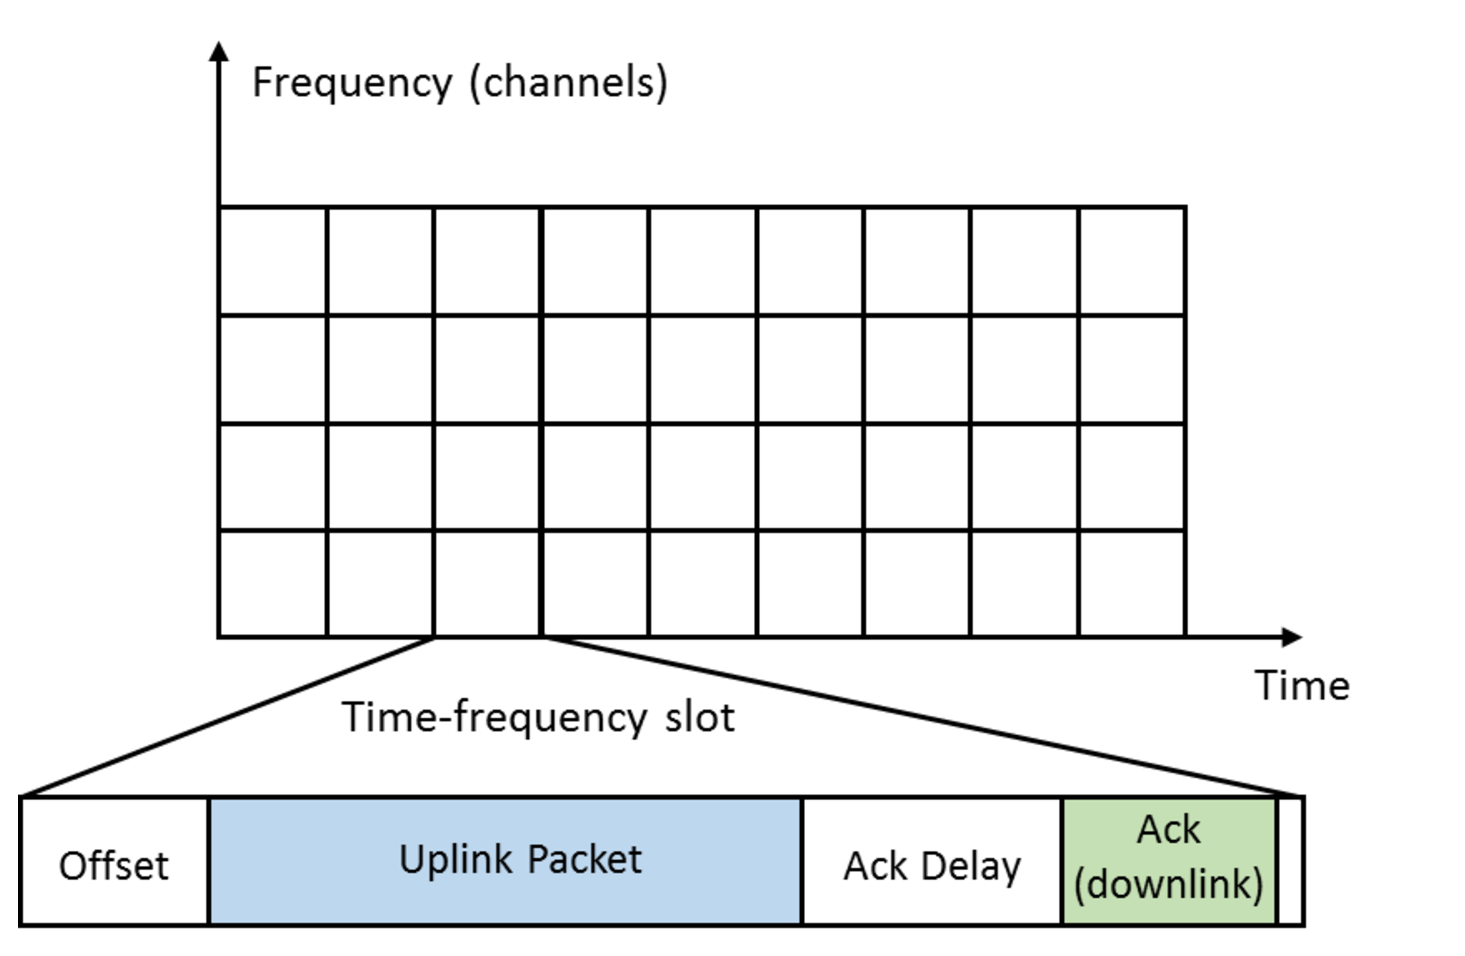
\includegraphics[height=0.35\textheight]{protocol.eps}\\
        
        {\small Chosen protocol : \textcolor{blue}{uplink messages {\large $\nearrow$}} followed by \textcolor{darkgreen}{\emph{acknowledgements} {\large $\searrow$}}.}\\
        \hfill{} {\tiny \textcolor{gray}{[Bonnefoi, Besson et al, CROWNCOM 2017], Sec.5.2}}
    \end{figure}

    \begin{itemize}
        % \tightlist
        \item
              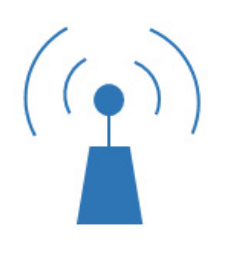
\includegraphics[height=0.37cm]{dynamic-devices.png} \(D\) \textbf{dynamic} devices trying to access the network
              \emph{independently}
        \item
              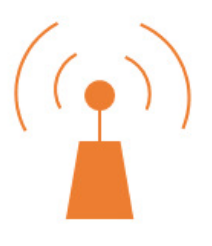
\includegraphics[height=0.37cm]{static-devices.png} \(S=S_1+\dots+S_{K}\) \textbf{static} devices occupying the network :
              \newline
              \(S_1,\dots,S_{K}\) in each channel \hfill{} (\emph{unknown}).
    \end{itemize}

\end{frameO}



\subsubsection{Hypotheses}

\begin{frameO}[Hypotheses ($1/2$)]

    \begin{colorblock}{Emission model for static and dynamic devices}

        \begin{itemize}
            % \tightlist
            \item
                  Each device has the same \emph{low} emission probability: \\
                  each step, each device sends a packet with probability \(p\).
                  \\
                  \hfill{}\small{(this gives a duty cycle proportional to $1/p$)}
        \end{itemize}

    \end{colorblock}

    \vspace*{20pt}

    \begin{lightblock}{Background ambiant traffic}

        \begin{itemize}
            % \tightlist
            \item
                  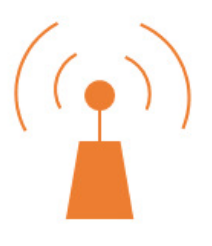
\includegraphics[height=0.37cm]{static-devices.png} Each static device uses only one channel
            \item
                  Their repartition is fixed in time \hfill{} $\implies$ \alert{stationary} hypothesis!
        \end{itemize}

        \(\implies\) This ambiant traffic \emph{is disturbing} the dynamic devices!
    \end{lightblock}

\end{frameO}

\begin{frameO}[Hypotheses ($2/2$)]

    \begin{colorblock}{Dynamic radio reconfiguration}

        \begin{itemize}
            % \tightlist
            \item
                Each \textbf{dynamic device decides} the channel to use to send every packet.
            \item
                It has memory and computational capacity to implement a basic decision algorithm.
        \end{itemize}

    \end{colorblock}

    \vspace*{20pt}

    \begin{lightblock}{Problem}

        \begin{itemize}
            % \tightlist
            \item
                  \emph{Goal} : \emph{maximize packet loss ratio} (\(=\) number of
                  received \texttt{Ack}) in a \emph{finite-space discrete-time Decision
                      Making Problem}.
            \item
                  \emph{Solution ?} \textbf{Multi-Armed Bandit algorithms},
                  \textbf{decentralized} and used \textbf{independently} by each device.
        \end{itemize}

    \end{lightblock}

\end{frameO}



\subsection{Baseline algorithms}

\subsubsection{$1)$ A naive strategy : uniformly random access}

\begin{frameO}[$1)$ A naive strategy : uniformly random access]

    \begin{itemize}
        % \tightlist
        \item
              \textbf{Uniformly random access}: dynamic devices choose uniformly
              their channel in the pull of \(K\) channels.
        \item
              Natural strategy, dead simple to implement.
    \end{itemize}

    \pause

    \begin{itemize}
        % \tightlist
        \item
            Simple analysis, in term of \textbf{successful transmission
            probability}\newline
            (for every message from dynamic devices) :
    \end{itemize}

    \begin{small} \begin{align*}
            \mathbb{P}(\text{success}|\text{sent}) = \sum_{k=1}^{K} \underbrace{(1 - p / K)^{D-1}}_{\text{No other dynamic device}} \times \underbrace{(1-p)^{S_k}}_{\text{No static device}} \times\; \frac{1}{K}.
        \end{align*} \end{small}

    \pause

    \begin{itemize}
        % \tightlist
        \item
              Works fine only if all channels are similarly occupied,\newline
              but \textbf{it cannot learn} to exploit the best (more free)
              channels.
    \end{itemize}

\end{frameO}



\subsubsection{$2)$ Optimal centralized strategy}

\begin{frameO}[$2)$ Optimal centralized strategy]

    \begin{itemize}
        % \tightlist
        \item
              If an oracle can decide to affect \(D_i\) dynamic devices to channel
              \(i\), the \textbf{successful transmission probability} is:
              \vspace*{-10pt}

              \begin{small} \begin{align*}
                      \mathbb{P}(\text{success}|\text{sent}) = \sum_{k=1}^{K} \underbrace{(1 - p)^{D_k - 1}}_{\;\;D_k - 1 \;\text{others}\;\;} \times \underbrace{(1 - p)^{S_k}}_{\;\;\text{No static device}\;\;} \times \underbrace{ D_k / D }_{\;\;\text{Sent in channel}\; i}.
                  \end{align*} \end{small}
              \pause
        \item
              The oracle has to solve this \textbf{optimization problem}:
              \vspace*{-5pt}

              \begin{small} \begin{equation*} \begin{cases}
                          \underset{D_1,\dots,D_{K}}{\arg\max}\;\;\; & \sum\limits_{k=1}^{K} D_k (1 - p)^{S_k + D_k -1}                                           \\
                          \text{such that}\;\;\;                     & \sum\limits_{k=1}^{K} D_k = D \; \text{and} \; D_k \geq 0, \; \; \forall 1 \leq k \leq K .
                      \end{cases} \end{equation*} \end{small}
        \item
              We solved this quasi-convex optimization problem with \emph{Lagrange
                  multipliers}, only numerically.
    \end{itemize}

    \vfill{}
    \(\implies\) It will have very good performance, as it maximizes the transmission rate
    of all the \(D\) dynamic devices.

\end{frameO}

\begin{frameO}[$2)$ Optimal centralized strategy]

    \begin{colorblock}{But unrealistic}

        But \textbf{not achievable in practice}:
        \begin{itemize}
            % \item
            % there is no oracle
            \item
                  \alert{because there is no centralized supervision!}
        \end{itemize}

    \end{colorblock}

    \vspace*{30pt}

    \begin{colorblock}{Let see \emph{realistic decentralized approaches}}

        \(\hookrightarrow\) Machine Learning ? \newline
        \hspace*{15pt}\(\hookrightarrow\) Reinforcement Learning ? \newline
        \hspace*{30pt} \(\hookrightarrow\) \emph{Multi-Armed Bandit} !

    \end{colorblock}

\end{frameO}



\begin{frameO}[Hum, what is a (one-armed )\emph{bandit}?]
    \begin{center}
        It's an old name for a casino machine!
    \end{center}

    \begin{center}
        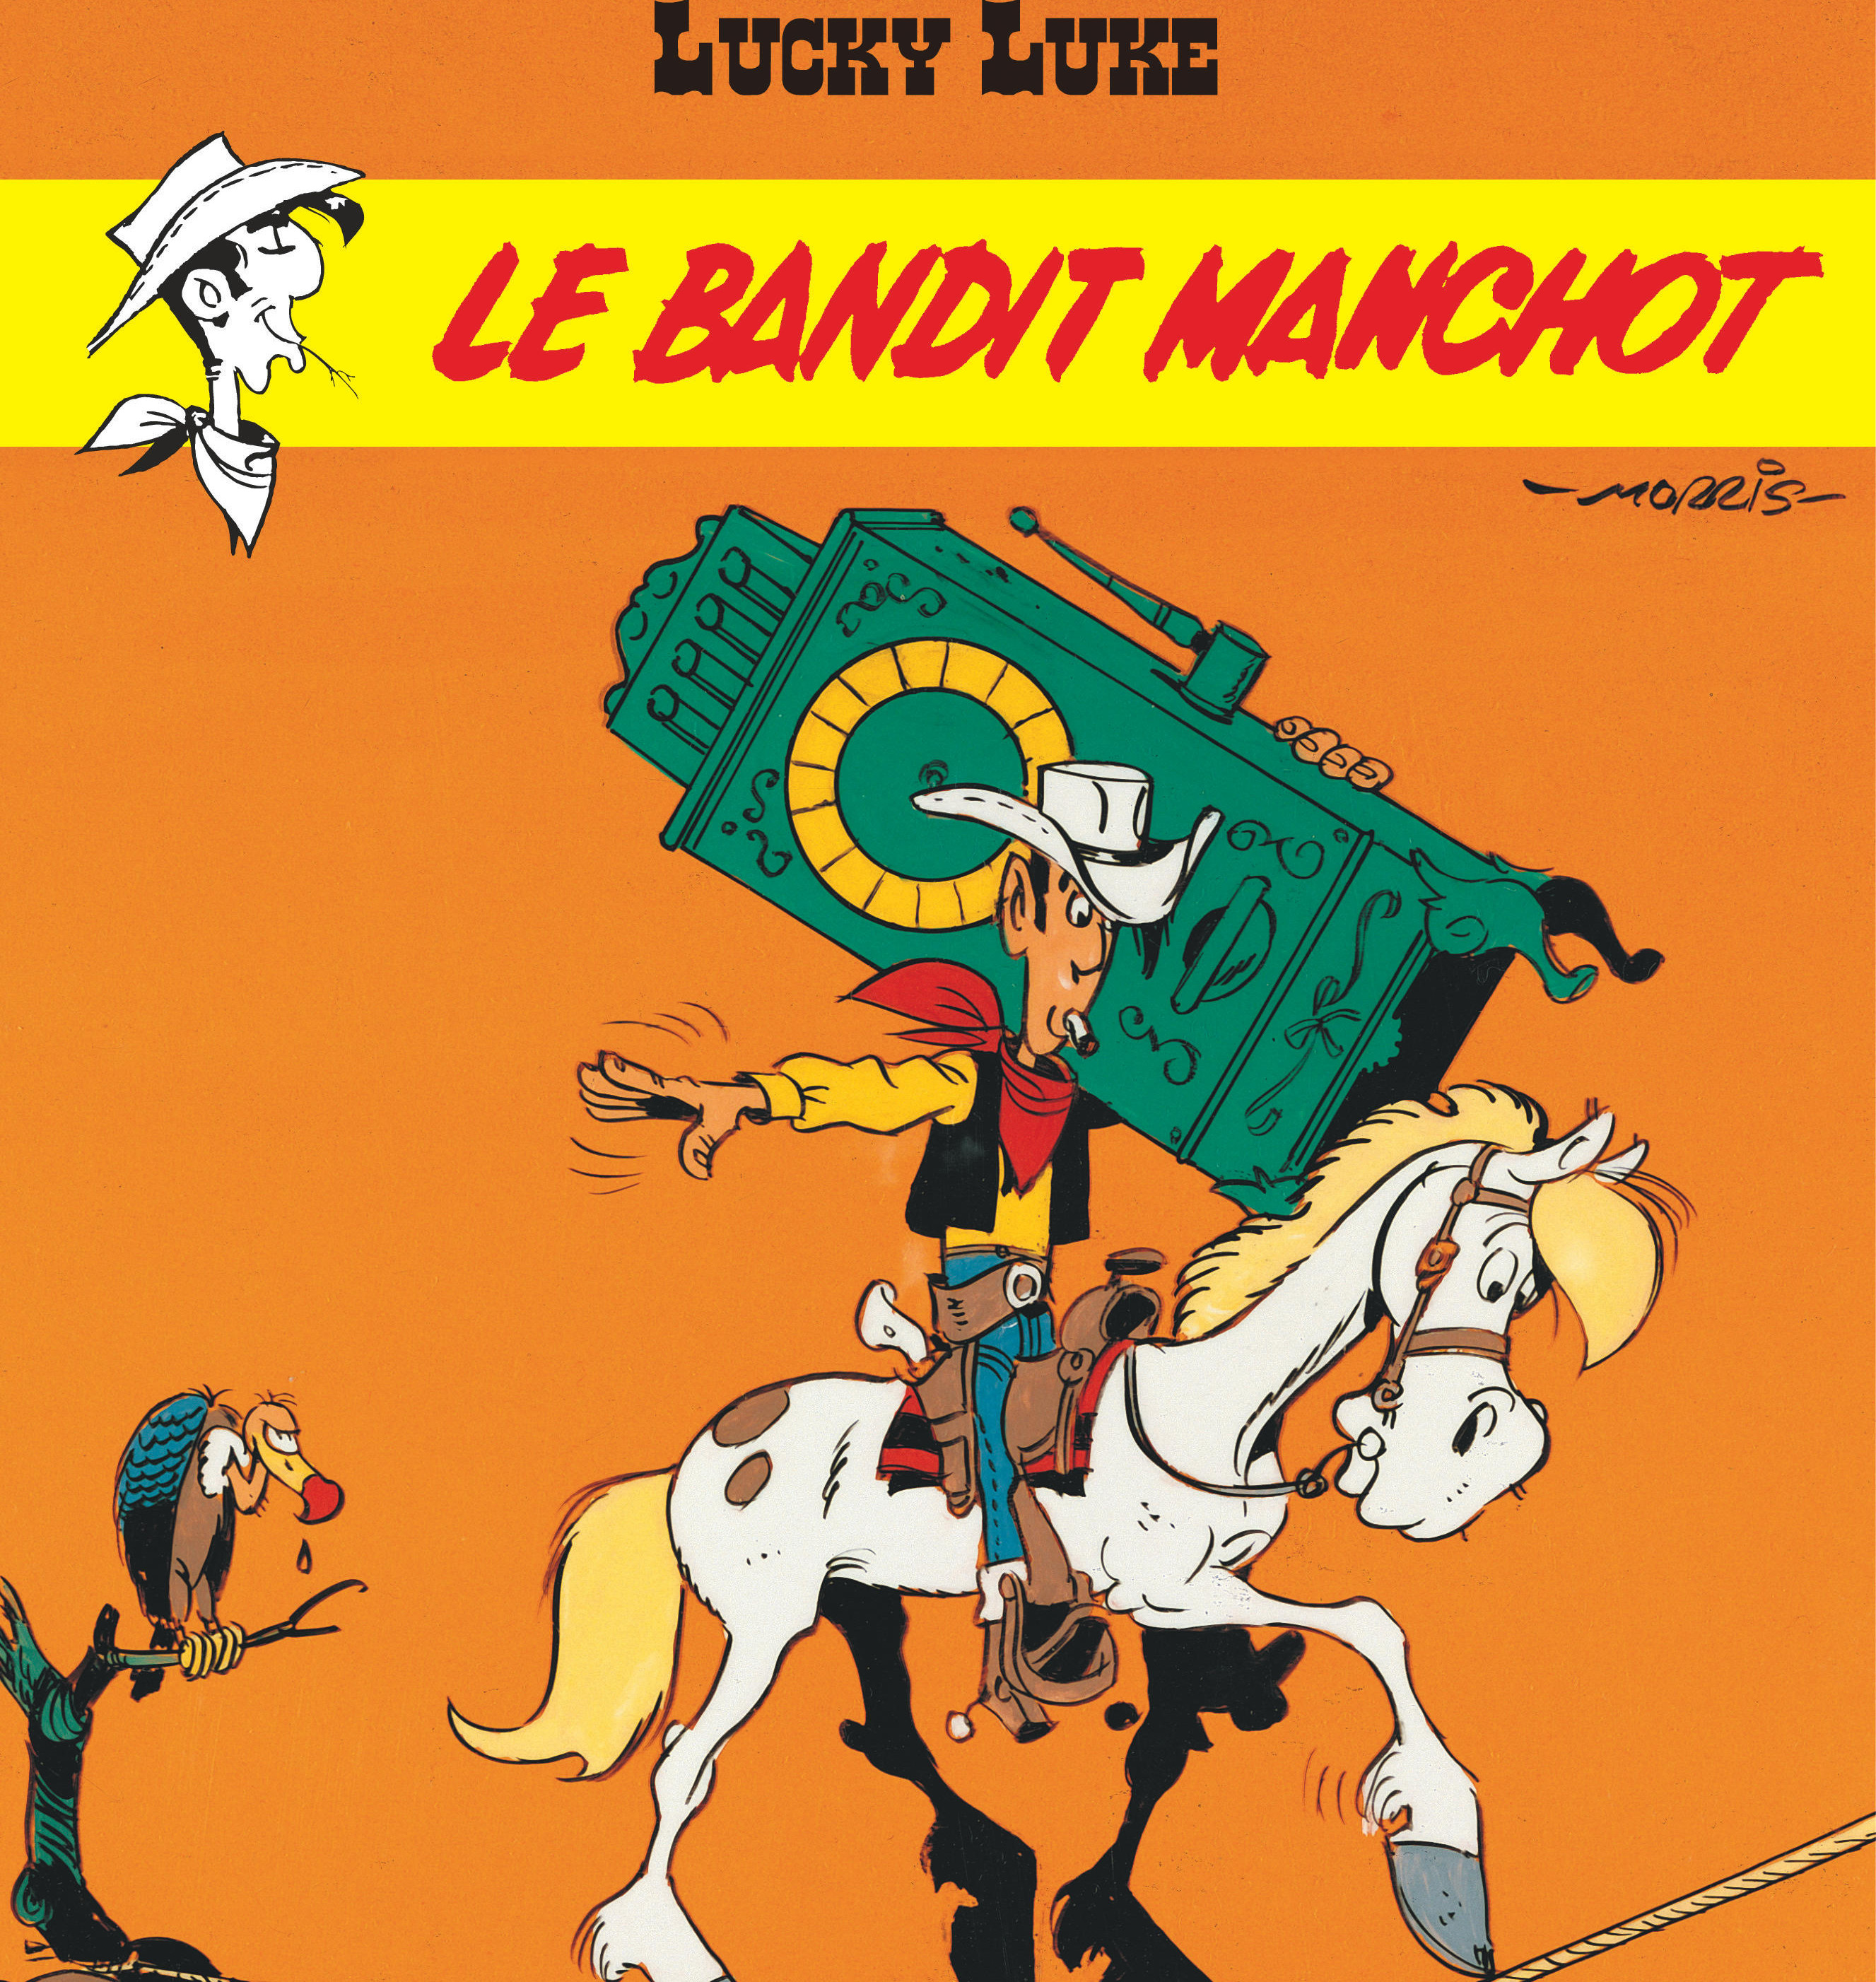
\includegraphics[height=6.5cm]{Lucky_Luke__Le_Bandit_Manchot.jpg}

        \begin{tiny}
            \textcolor{gray}{
                \textcopyright{} Dargaud,
                \href{https://www.dargaud.com/bd/LUCKY-LUKE/Lucky-Luke/Lucky-Luke-tome-18-Bandit-manchot-Le}{\textcolor{blue}{Lucky Luke tome 18}}.
            }
        \end{tiny}
    \end{center}
\end{frameO}



\subsection{Multi-Armed Bandit algorithm : UCB}

\subsubsection{Multi-Armed Bandit formulation}

\begin{frameO}[$3)$ \emph{Multi-Armed Bandit} formulation]

    A dynamic device tries to collect \emph{rewards} when transmitting :

    \begin{itemize}
        % \tightlist
        \item
            it transmits following a random Bernoulli process \newline
            (of probability \(p\) of transmitting at each time step \(t\)),
        \item
            it chooses a channel \(A(\tau) \in \{1,\dots,K\}\)
            \hfill{} ($=$ arm \slotmachine)
        \item
            if \texttt{Ack} (no collision) \hspace*{2pt} \(\implies\) reward
            \(r_{A(\tau)} = 1\) \hfill{} (successful transm.!)
        \item
            if collision (no \texttt{Ack}) \hspace*{2pt} \(\implies\) reward
            \(r_{A(\tau)} = 0\) \hfill{} (failed transmission!)
    \end{itemize}

    \vfill{}

    \begin{colorblock}{Reinforcement Learning interpretation}

        Maximize transmission rate \(\equiv\) \textbf{maximize cumulated rewards}
        \[\max_{\text{algorithm}\;A} \;\; \sum_{\tau=1}^{\text{horizon}} r_{A(\tau)}.\]

    \end{colorblock}

\end{frameO}

\subsubsection{Upper Confidence Bound algorithm : UCB}

\begin{frameO}[$3)$ Upper Confidence Bound algorithm (\(\mathrm{UCB}_1\))]

    \only<1-2>{
        A dynamic device keeps \(\tau\) number of sent packets, \(N_k(\tau)\)
        selections of channel \(k\), \(X_k(\tau)\) successful transmission in
        channel \(k\).
    }

    \begin{enumerate}
        \def\labelenumi{\arabic{enumi}.}

        % \tightlist
        \only<1-2>{
            \item
              For the first \(K\) activations (\(\tau=1,\dots,K\)), try each channel
              \emph{once}.
        }
        \pause
        \item
              Then for the next steps \(t\) :

              \begin{itemize}
                  % \tightlist
                  \item
                        With probability $p$, the device is active ($\tau := \tau + 1$)
                \only<1-2>{
                  \item
                        Compute the index
                        \(\mathrm{UCB}_k(\tau) := \overbrace{\frac{X_k(\tau)}{N_k(\tau)}}^{\text{Mean}\; \widehat{\mu_k}(\tau)} + \overbrace{\sqrt{\frac{\log(\tau)}{2 N_k(\tau)}},}^{\text{Upper Confidence Bound}}\)
                  \item
                        Choose channel
                        \(A(\tau) = \mathop{\arg\max}\limits_{k} \; \mathrm{UCB}_k(\tau)\),
                  \item
                        Update \(N_k(\tau+1)\) and \(X_k(\tau+1)\),
                }
                \only<3>{
                    \item \dots{}
                }
                  \item
                        Wait for next message\dots \hfill{} (mean waiting time $\simeq 1/p$)
              \end{itemize}
    \end{enumerate}

    \only<3>{
    \begin{colorblock}{Random activation?}
        \begin{itemize}
            \item
                  The times $\tau$ are \textbf{not} the global time indexes $t$
            \item
                  each object transmits only with probability $p$ at each time $t$
            \item
                  following its Bernoulli activation pattern
        \end{itemize}
        \alert{$\implies$ all the random activations make the model intractable in theory!}
    \end{colorblock}
    }

    % \vfill{}\hfill{}\tiny{\textcolor{gray}{References: [Lai \& Robbins, 1985], [Auer et al, 2002], [Bubeck \& Cesa-Bianchi, 2012]}}

\end{frameO}



\subsection{Experimental results}

\subsubsection{Experiment setting}

\begin{frameO}[Experimental setting]

    \begin{colorblock}{Simulation parameters}

        \begin{itemize}
            \setlength\itemsep{10pt}
                  % 
                  % \tightlist
            \item
                  \(K = 10\) channels,
            \item
                  \(S + D = 10000\) devices in total,
            \item
                  \(p = 10^{-3}\) probability of emission,
            \item
                  Horizon \(T = 10^5\) total time slots (avg. \(\simeq 100\) messages \(/\)
                  device),
            \item
                  The proportion of 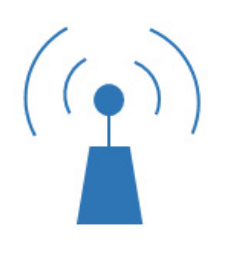
\includegraphics[height=0.37cm]{dynamic-devices.png} dynamic devices \(D/(S+D)\) varies,
            \item
                  Various settings for 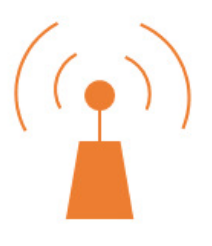
\includegraphics[height=0.37cm]{static-devices.png}  \((S_1,\dots,S_{K})\) static devices repartition.
        \end{itemize}

    \end{colorblock}

\end{frameO}



\subsubsection{First result: $10\%$}

\begin{frameO}[\(10\%\) of dynamic devices]

    \begin{figure}[h!]
        \centering
        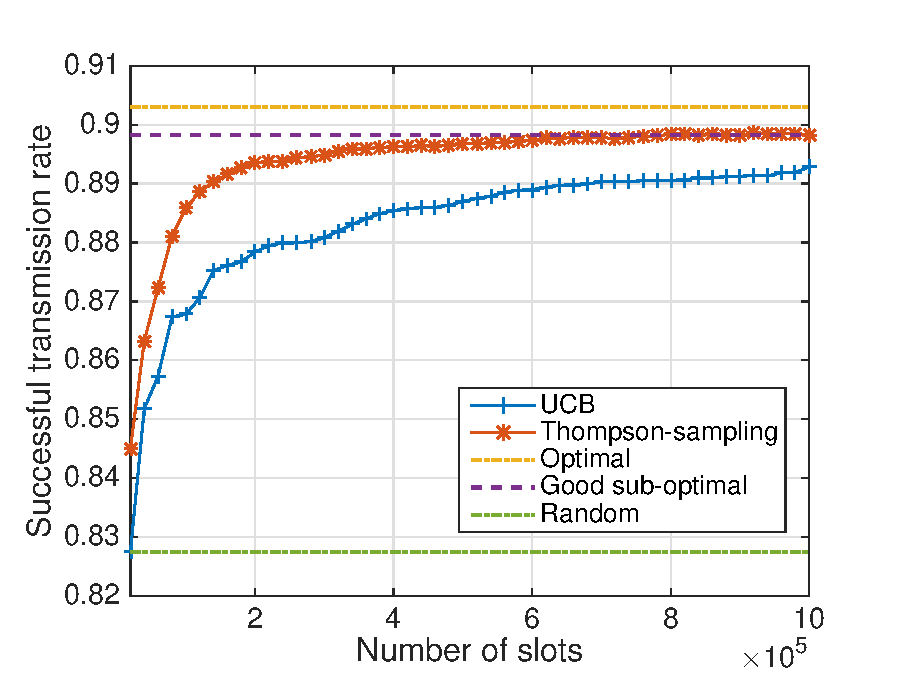
\includegraphics[height=0.74\textheight]{10intelligent.eps}

        % \caption{
            $10\%$ of dynamic devices. Gives $7\%$ of gain.\\
            {\tiny \textcolor{gray}{[Bonnefoi, Besson et al, CROWNCOM 2017], Sec.5.2}}
        % }
    \end{figure}

\end{frameO}



\subsubsection{First result: $30\%$}

\begin{frameO}[\(30\%\) of dynamic devices]

    \begin{figure}[h!]
        \centering
        \includegraphics[height=0.74\textheight]{30intelligent.eps}

        % \caption{
            \begin{small}
                $30\%$ of dynamic devices. Gives $3\%$ of gain but not much is possible here.
            \end{small}
        % }
    \end{figure}

\end{frameO}


\subsubsection{Growing proportion of devices dynamic devices}

\begin{frameO}[Dependency on \(D/(S+D)\)]

    \begin{figure}[h!]
        \centering
        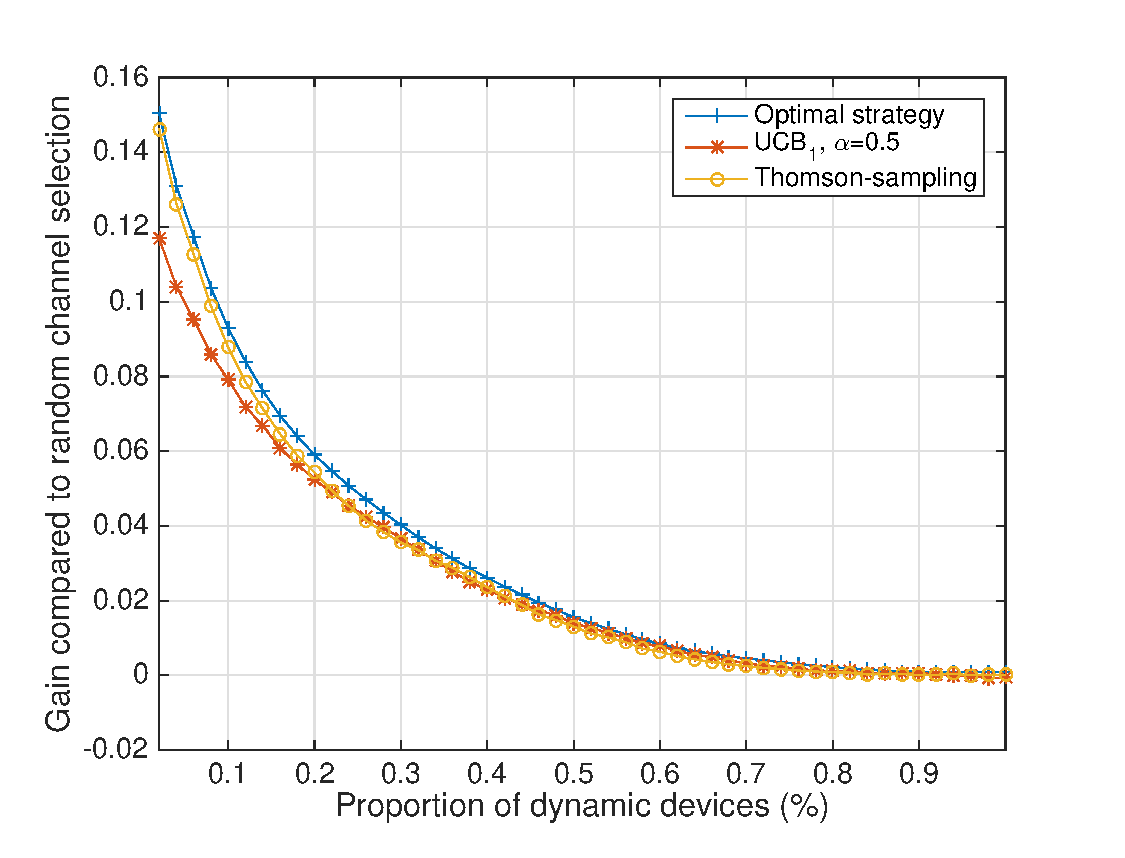
\includegraphics[height=0.70\textheight]{perf_learning.eps}

        % \caption{
            \emph{Almost optimal}, for any proportion of dynamic devices, \emph{after a short learning time}. Up-to $16\%$ gain over the naive approach!
        % }
    \end{figure}

\end{frameO}


\begin{frameO}[\emph{Positive} conclusion from experiments ($1/2$)]

    \begin{colorblock}{What do we show}

        \begin{itemize}
            \setlength\itemsep{10pt}
                  % \tightlist
            \item
                  After a short learning time, MAB algorithms are almost as efficient as
                  the oracle solution
            \item
                  Never worse than the naive solution, even at first iterations
            \item
                  Thompson sampling is more efficient than UCB
                  (as always)
            \item
                  The dynamic devices can learn to communicate more efficiently,\\
                  in any network configuration (we tried a lot more!)
        \end{itemize}

    \end{colorblock}

\end{frameO}


% \begin{frameO}[\emph{Negative} conclusion from experiments ($2/2$)]

%     \begin{lightblock}{But what are the limitations?}

%         \begin{itemize}
%             \setlength\itemsep{5pt}
%                   % \tightlist
%             \item
%                 \textcolor{orange}{\textbf{Only works empirically}!}
%                 \\
%                 Theoretically, we showed counter examples where the \textbf{Selfish} approach can fail, for the smallest case $D = 2$ devices, $p=1$ in $K=3$ channels
%             \item
%                 $p \times (D + S)$ devices in $K$ channels in average\\
%                 $\implies$ $p \ll \frac{K}{(D + S)}$ gives best performance
%             \item
%                 Only works empirically with a stationary hypothesis on the background traffic\dots
%             \item
%                 \textbf{Intractable model} in theory, mainly due to too much randomness (activations, collisions, selections\dots)
%         \end{itemize}

%     \end{lightblock}

% \end{frameO}
